\documentclass{scrreprt}
\usepackage{enumitem}
\usepackage{listings}
\usepackage{underscore}
\usepackage[ddmmyyyy]{datetime}
\renewcommand{\dateseparator}{--}
\usepackage[bookmarks=true]{hyperref}
\usepackage[utf8]{inputenc}
\usepackage[english]{babel}
\usepackage{url}
\usepackage{graphicx}

\newenvironment{enum}
{\begin{enumerate}[label*=\arabic*.][resume]}
{\end{enumerate}}

\hypersetup{
    bookmarks=false,    % show bookmarks bar?
    pdftitle={Software Requirement Specification},    % title
    pdfauthor={John Zlotek},                     % author
    pdfsubject={TeX and LaTeX},                        % subject of the document
    pdfkeywords={TeX, LaTeX, graphics, images}, % list of keywords
    colorlinks=true,       % false: boxed links; true: colored links
    linkcolor=blue,       % color of internal links
    citecolor=black,       % color of links to bibliography
    filecolor=black,        % color of file links
    urlcolor=purple,        % color of external links
    linktoc=page            % only page is linked
}%
\def\myversion{2.0.0 }
\date{}
%\title
\usepackage{hyperref}
\begin{document}

\begin{flushright}
    \rule{16cm}{5pt}\vskip1cm
    \begin{bfseries}
        \Huge{SOFTWARE REQUIREMENTS\\ SPECIFICATION}\\
        \vspace{1.0cm}
        for\\
        \vspace{1.0cm}
        Checkers\\
        \vspace{1.5cm}
        \LARGE{Version \myversion approved}\\
        \vspace{1.5cm}
        Prepared by:\\
    John Zlotek\\
    Matt Horger\\
    Jake Carfagno\\
    Preet Patel\\
        \vspace{1.9cm}
        Team: \textbf{Big Chungus}\\
        \vspace{1cm}
        \today\\
    \end{bfseries}
\end{flushright}

\tableofcontents

\chapter*{Revision History}

\begin{center}
    \begin{tabular}{|c|c|c|c|}
        \hline
        Name & Date & Reason For Changes & Version\\
        \hline
        1.0.0 & \formatdate{11}{7}{19} & Initial Structure & mhorger, jzlotek\\
        \hline
        1.0.1 & \formatdate{17}{7}{19} & More Structure & mhorger, jzlotek\\
        \hline
        1.1.0 & \formatdate{18}{7}{19} & User Interface & jcarfagno\\
        \hline
        1.1.1 & \formatdate{20}{7}{19} & Introduction Information & ppatel\\
        \hline
        2.0.0 & \formatdate{22}{7}{19} & Final Submission & mhorger\\
        \hline
    \end{tabular}
\end{center}

\chapter{Introduction}

\section{Purpose of Document}
The purpose of the requirement specification is to outline the state-of-the-art
web-based Checker game. This game will allow multiple players to interact
with each other through a client-server-client manner, it allows them to play
and chat. This document covers the scope, objective, basic requirement and
goal for this new game. Apart from that this document also covers a topic in-
depth like functional, non-functional, user interface design, test cases,
program usage, and references. The intention here to make end-user or an
engineer understand the design and implantation of this game.

\section{Project Scope}
The purpose of this document is to educate the reader thoroughly about this
game, how it works, what’s been used, and to lay out the requirements of the program itself.

\section{Overview of Document}
This document contains all general explanation about technology, software
work and why they are implemented. Here the document also outlines and
describe the specific components of this project. As far as sequence goes, it
starts with functional requirement which goes over in two major parts –
Server and Client, followed by non-functional requirement which covers
networking components and system requirements, then it goes over front end
of the project like user interface which goes over framework, menus, and
standard components, it also has outlined program usage which includes
lobbies, gameplay and wining conditions and finally document ending with references.

\section{Background}

\subsection{History}

There have been many instances in history where the concept of checkers has been found. The earliest was as far as 3000 B.C
in ancient Iraq and then in 1400 B.C in ancient Egypt using a 5X5 board \cite{historyCheckers}. 
The game we know today was developed in the mid 1500s as an English mathematician developed the rules on what was known as Draughts in 1756, adapting many of the similar mechanics from a Frenchman 400 years earlier. Over time, this game developed to be one of the most popular classic board games of all time.

\subsection{Game Rules}
	These rules are adapted from the American Checker Federation \cite {checkersFoundation}.
	\begin{enumerate}
	\item Red always gets to play first.
	\item A player can forfeit at any time, conceding victory to the other player.
	\end{enumerate}
\subsubsection{Moves} 
\begin{enumerate}
    \item A player may only move their own pieces.
    \item Normal Piece
        \subitem A normal piece may only move toward the other player's side of the board.
        \subitem A normal piece may move diagonally to the left or right to a vacant square in front of it.
        \subitem A normal piece may capture on the diagonal if there exists a vacant square one more diagonal position ahead.
            \subsubitem A piece may move again if there exists another piece to capture after making a capture.
    \item A King Piece moves the same as a normal piece but can move and capture backward.
    \item A King Piece may capture forward or backward.
    \item If a normal piece reaches the opposite edge of the board, it becomes a King Piece.
\end{enumerate}

\subsubsection{Win Condition}
\begin{enumerate}
    \item When one player has no more pieces to move, the other player is the winner.
    \item If a player forfeits the match, the other player is conceded the winner.
\end{enumerate}

\section{Abstract}

We believe that this document will serve any team member currently or in the future enough requirement to build both a client-facing and server application in order to play checkers.
By constructing our game engine, we will be able to host any amount of games for an infinite amount of clients to enjoy the classic game of checkers. As for the timeline of this class, CS 451, we hope to implement all of the following requirements and specifications listed out below in detail. 

\chapter{Overall Description}

\section{Product Functions}

\begin{enumerate}
    \item Provide a client-facing application to play checkers with another user over the local network or internet.
    \item Provide a centralized server that mediates gameplay, game sessions, and client interactions.
    \item Provide enough documentation that future team members can pickup the product from scratch and improve on it.
\end{enumerate}

\section{Assumptions and Dependencies}

\begin{enumerate}
    \item A connection to a local network where the server is hosted or internet connection.
    \item A computer with a graphical windowing environment for the client and any *nix or Windows based server.
    \item Client who have some knowledge of the rules of checkers and how to play either previously or by looking at our requirements documentation.
    \item Client know how to launch a .JAR file from a desktop and interact with simple menu components.
\end{enumerate}

\chapter{Functional Requirements}

\section{Client}

\begin{enumerate}[label*=R\arabic*.]
    \item Client - Server Interaction
    \begin{enumerate}[label*=\arabic*.]
        \item Client will automatically check to see if the game server is live given the set URL in the program.
        \item Client will not be able to join a lobby if no response is sent from the requested server URL.
        \item Client will be able to terminate itself from the server at any given moment.
        \item Client will be able to reconnect back to the lobby within 30 seconds, else they will receive a notification saying that the lobby has been closed and they are unable to rejoin due to the timeout period.
        \item Client will be able to see all available games to join on the server and be able to select a lobby.
        \item Client should be able to distinguish themselves with a valid player name when they join a lobby.
        \item Clients will be able to select which color they want to play, and receive the assigned color once the game begins.
    \end{enumerate}
\end{enumerate}

\subsection{Board State}

\begin{enumerate}[resume*]
    \item Board
    \begin{enumerate}[label*=\arabic*.]
        \item The clients will keep a copy of the board state in order to render it
        \item The board will update upon receiving an input from either:
            \subitem Server response
    \end{enumerate}
\end{enumerate}

\section{Server}

\begin{enumerate}[resume*]
    \item Server should be able to be run all the time without crashing.
        \subitem Server will have a heartbeat function that will send an email to the developers if the server is down for some reason.
    \item Server - Client Interaction
    \begin{enumerate}[label*=\arabic*.]
        \item Server will be able to process client connection information to create a lobby.
        \item Server will keep track of clients and game sessions.
        \item On user timeout, wait a set amount of time.
            \subitem If not connected within that time, signal other client game has ended due to disconnected player.
        \item Server will validate moves before sending updated move to clients.
            \subitem On invalid move, signal client that move was invalid and to try again.
    \end{enumerate}
    \item Server - Lobby Interaction
    \begin{enumerate}[label*=\arabic*.]
        \item Server has a fixed range of ports that it can assign a lobby upon creation. This range is to make sure we do not flood our network with ports ranging far away from each other.
        \item Server will first check that a port is open before assigning it to a lobby upon creation.
        \item Server will close the port assigned to a lobby when the game has been finished.
        \item Server will be able to print out a list of lobbies for the clients to see.
        \item Server will be able to send notice to any lobbies that the server is shutting down, whether expectedly or unexpectedly, in order to provide better experience for the clients playing.   
    \end{enumerate}
\end{enumerate}

\chapter{Other Requirements}

\section{System Requirements}

\begin{enumerate}[label*=S\arabic*.]
    \item Server and Client
        \subitem JRE Version 12 or higher
    \item Client
        \subitem Windowing display environment:
            \subsubitem Windows
            \subsubitem MacOS
            \subsubitem Xorg or Wayland
\end{enumerate}

\section{Network Requirements}

\begin{enumerate}[label*=N\arabic*.]
    \item Client and Server
	 \begin{enumerate}[label*=\arabic*.]
        \item An active internet connection is required for the client to connect to the server.
        \item Client cannot download the server and run it locally, unless the client sets up port forwarding properly on their local network.
        \item Client must be connected to Drexel's network in order to play. This requires credentials to sign-in. Client is responsible for their own Drexel credentials. 
        \item Response time to the server must be less than 120ms. If it is greater, then the game quality may be decreased and we will alert the clients.
	  \end{enumerate}
    \item Server
 	\begin{enumerate}[label*=\arabic*.]
        \item Server must be hosted on tux.cci.drexel.edu. We are at the mercy of tux.cci.drexel.edu's uptime.
        \item Server will be running on one dedicated box, and will not have a load balancer assigned to it, meaning that there will be one direct access point for our clients to connect to.
        \item There will be no snapshots saved of the server or gamestates. Server will have little to no storage to save information to load back onto the network.
        \item If a client is taking too long to connect, the server will automatically ditch the requested connection.
  \end{enumerate}
\end{enumerate}

\chapter{User Interface}

\section{Framework}

The project shall use JavaFX to create the user interface. We shall write a wrapper for it to facilitate ease of use.

\section{Menus}

\begin{itemize}
\item Main Menu
    \subitem Play Game button: connects player to the server to search for a match, moving them to the Game Lobby screen
    \subitem Quit Game: closes the game

\item Game Lobby
    \subitem Show one (or both) players in the lobby
    \subitem Ready? button: start game once both players click
    \subitem Main Menu button: return to the main menu

\item Game
    \subitem Checkers match screen, showing a checkers board with both players’ pieces
        \subsubitem Player’s “side” of the board is always the bottom from their own perspective, mirroring real-life players sitting on opposite sides of a board
    \subitem Top of screen shows whose turn it is: Black or Red
        \subsubitem During the player’s turn, they click on a piece to select it
        \subsubitem Piece becomes highlighted, as does all valid spaces the player could move to
        \subsubitem Player clicks on a highlighted space to move the piece there or clicks on a new piece to select it
        \subsubitem After a move has been made, the game checks if there is a winner. Move to Winner Display if a winner is found. Otherwise, start next player’s turn.

\item Winner Display
    \subitem Show the player who won the game: Black or Red
    \subitem Rematch? No button: return both players to the main menu
    \subitem Rematch? Yes button: register this player as wanting a rematch
        \subsubitem If both players click Yes, then return both players to the Game Lobby screen
\end{itemize}

\section{Standard Components}

\begin{itemize}
    \item Buttons: The buttons will be used for interaction within menus, allowing for navigation throughout the program.
    \item Pieces (Black and Red variants): The pieces will be the basic playing pieces within gameplay. Clicking on a piece will select it for making a move during the player’s turn.
    \item King Pieces (Black and Red variants): These pieces will behave identically to the regular pieces (see above) but with additional movement options according to the rules of Checkers.
    \item Checkers Board: an 8x8 grid of alternating black and red tiles on which all pieces will be displayed in the gameplay. When a piece is selected during a player’s turn, all spaces to which the player could move will be highlighted. Clicking on a highlighted space will move the piece to that space, jumping over any opponent pieces if possible.
\end{itemize}

\chapter{Program Usage}

\section{Lobbies}
\begin{enumerate}[label*=L\arabic*.]
    \item Lobby Creation    
        \begin{enumerate}[label*=\arabic*.]
            \item Clients should be able to create a lobby (start a new game) or join a lobby (join another player to start a game).
                \subitem When a client creates a lobby, this opens a port on the server.
                \subitem When a client joins a lobby, the game then starts processing the pre-game information.
                \subitem Information in the pre-game is the names of the players, who is selected to play which color, and which client goes first (the client assigned to the red color).
        \end{enumerate}
    \item Lobby Rules
        \begin{enumerate}[label*=\arabic*.]
            \item Lobbies consist of a number of players, whether or not the game is started or finished, and what port it is being hosted on the server.
                \subitem A player can join a lobby via the port number, as this acts as our identity for each lobby.
            \item There will be a maximum of 10 lobbies that the server will allow in order not to crash the server.
            \item Lobbies will be locked down once two clients have connected.
                \subitem If a third client tries to connect to a game-in-progress, an alert will be sent to that user saying "spectating is not allowed for a game-in-progress".
            \item If the server were to crash, all lobbies will be terminated without any winners assigned.
            \item A lobby can only be initialized when a player creates one. There will be no default lobbies maintained by the server.
            \item A lobby will only be assigned to a given range of ports from the server. This is to make sure that the ports are available for creation.                         
        \end{enumerate}
\end{enumerate}

\section{Gameplay}
\begin{enumerate}[label*=G\arabic*.]
	\item The match begins with an 8x8 grid with each tile alternating between black and red in color.
	\item One player is assigned the black pieces and the other red.
	\item Each player’s pieces start on opposite ends of the board, occupying every other space within the first three rows (for a total of 12 pieces for each player).
	\subitem See attached image for an example checkers setup:
	\subitem 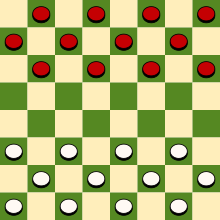
\includegraphics[width=8cm]{board.png}
	\item The black player starts the match by taking their turn.
	\item During each turn, the active player selects a piece of their own to move according to the following rules:
\begin{itemize}
    \item If the piece is bordering an enemy piece and there is a free space on the other side of that enemy piece, the piece must “jump” to the empty space, removing the enemy piece it moved over from the board
        \subitem Multiple jumps can be made in a single turn if the piece is in position to jump an additional enemy piece after completing a jump
    \item If the piece cannot jump, it may move diagonally one space to an unoccupied space
        \subitem If the piece is a non-king, it must move forward
        \subitem If the piece is a king, it can move in any direction
    \item A piece cannot jump over pieces of the same color as itself (friendly pieces)
    \item Two pieces cannot occupy the same space, regardless of color
\end{itemize}

\item When a non-king piece has reached the edge of the board opposite its color’s starting side, that piece will be crowned and turned into a king, allowing it to move in any direction.
\end{enumerate}
\subsection{Win Conditions}

\begin{enumerate}
    \item If player A has no more pieces, player B is the winner and vice versa.
    \item If player A disconnects, player B is the winner and vice versa.
\end{enumerate}


\begin{thebibliography}{9}

\bibitem{checkersFoundation}
  The American Checker Foundation,
  \textit{USA Checkers},
  https://www.usacheckers.com/,
  2019.

\bibitem{historyCheckers}
W.J. Rayment,
\textit{History of Checkers or Draughts},
http://www.indepthinfo.com/checkers/history.shtml,
2004.

\end{thebibliography}


\end{document}
